\documentclass{standalone}
\usepackage{tikz}
\usetikzlibrary{patterns}
\usetikzlibrary{positioning}
\usetikzlibrary{patterns, positioning}
\usetikzlibrary{shapes.misc}
\usepackage[outline]{contour}
\contourlength{1.5pt} 
\usepackage[sfdefault]{ClearSans}

\begin{document}
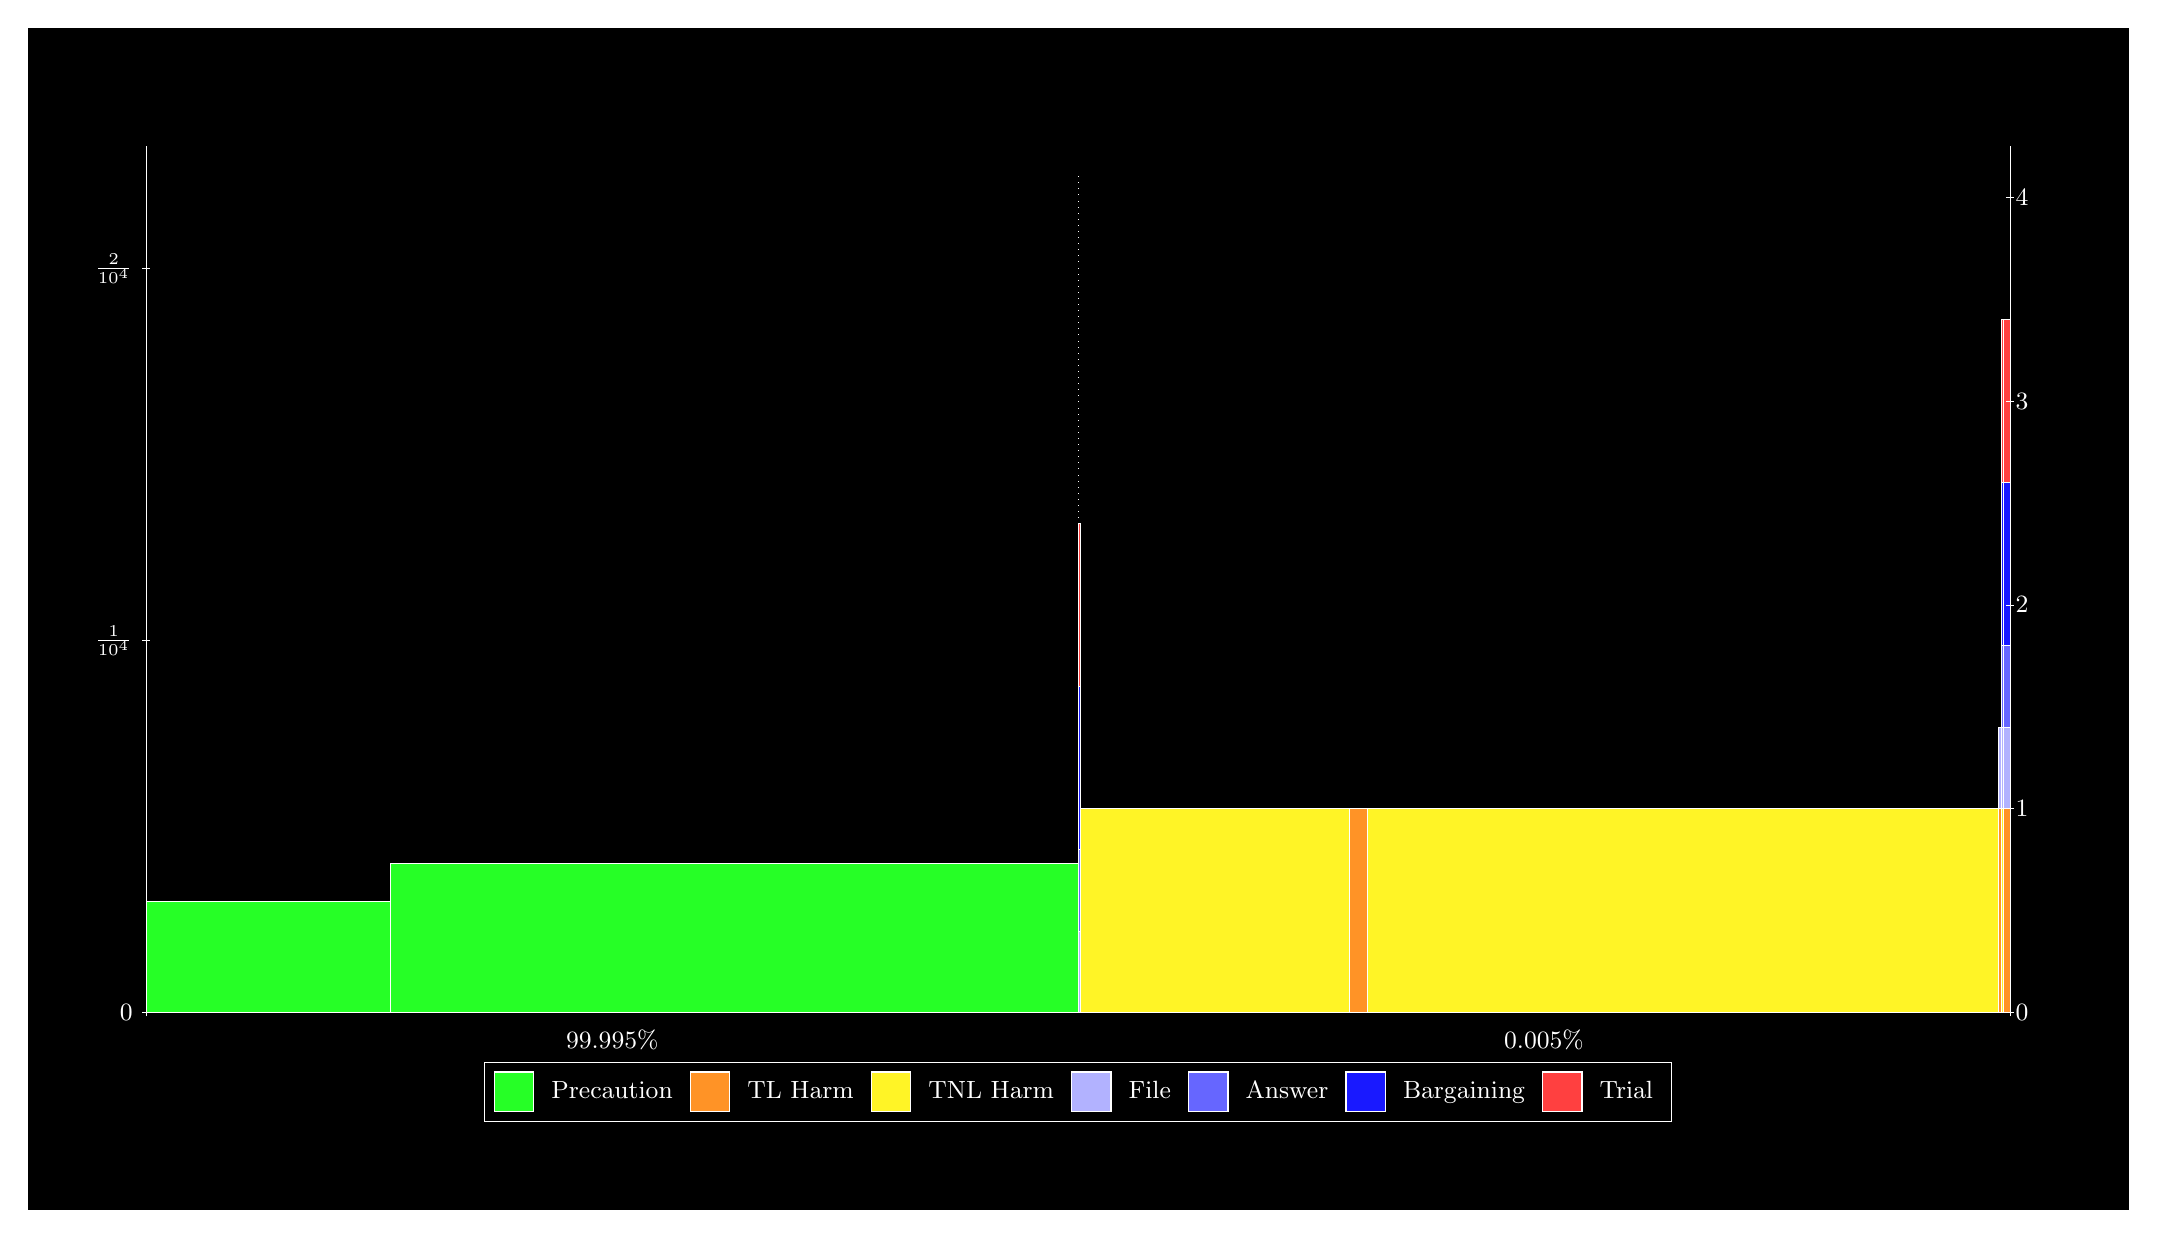
\begin{tikzpicture}
\draw[fill=black] (0,0) rectangle (26.667,15);
\draw[fill=green!85,draw=white,very thin] (1.5,2.5) rectangle (4.5937,3.9173);
\draw[fill=green!85,draw=white,very thin] (4.5937,2.5) rectangle (13.333,4.3898);
\draw[fill=green!85,draw=white,very thin] (13.333,2.5) rectangle (13.34,2.5001);
\draw[fill=blue!30,draw=white,very thin] (13.333,2.5001) rectangle (13.34,3.5354);
\draw[fill=green!85,draw=white,very thin] (13.34,2.5) rectangle (13.361,2.5001);
\draw[fill=blue!30,draw=white,very thin] (13.34,2.5001) rectangle (13.361,3.5354);
\draw[fill=blue!60,draw=white,very thin] (13.34,3.5354) rectangle (13.361,4.5706);
\draw[fill=blue!90,draw=white,very thin] (13.34,4.5706) rectangle (13.361,6.6412);
\draw[fill=red!75,draw=white,very thin] (13.34,6.6412) rectangle (13.361,8.7118);
\draw[fill=green!85,draw=white,very thin] (13.361,2.5) rectangle (16.773,2.5001);
\draw[fill=yellow!85,draw=white,very thin] (13.361,2.5001) rectangle (16.773,5.0883);
\draw[fill=green!85,draw=white,very thin] (16.773,2.5) rectangle (17.012,2.5001);
\draw[fill=orange!85,draw=white,very thin] (16.773,2.5001) rectangle (17.012,5.0883);
\draw[fill=green!85,draw=white,very thin] (17.012,2.5) rectangle (25.016,2.5001);
\draw[fill=yellow!85,draw=white,very thin] (17.012,2.5001) rectangle (25.016,5.0883);
\draw[fill=green!85,draw=white,very thin] (25.016,2.5) rectangle (25.022,2.5001);
\draw[fill=yellow!85,draw=white,very thin] (25.016,2.5001) rectangle (25.022,5.0883);
\draw[fill=blue!30,draw=white,very thin] (25.016,5.0883) rectangle (25.022,6.1236);
\draw[fill=green!85,draw=white,very thin] (25.022,2.5) rectangle (25.054,2.5001);
\draw[fill=orange!85,draw=white,very thin] (25.022,2.5001) rectangle (25.054,5.0883);
\draw[fill=blue!30,draw=white,very thin] (25.022,5.0883) rectangle (25.054,6.1236);
\draw[fill=green!85,draw=white,very thin] (25.054,2.5) rectangle (25.088,2.5001);
\draw[fill=yellow!85,draw=white,very thin] (25.054,2.5001) rectangle (25.088,5.0883);
\draw[fill=blue!30,draw=white,very thin] (25.054,5.0883) rectangle (25.088,6.1236);
\draw[fill=blue!60,draw=white,very thin] (25.054,6.1236) rectangle (25.088,7.1589);
\draw[fill=blue!90,draw=white,very thin] (25.054,7.1589) rectangle (25.088,9.2294);
\draw[fill=red!75,draw=white,very thin] (25.054,9.2294) rectangle (25.088,11.3);
\draw[fill=green!85,draw=white,very thin] (25.088,2.5) rectangle (25.167,2.5001);
\draw[fill=orange!85,draw=white,very thin] (25.088,2.5001) rectangle (25.167,5.0883);
\draw[fill=blue!30,draw=white,very thin] (25.088,5.0883) rectangle (25.167,6.1236);
\draw[fill=blue!60,draw=white,very thin] (25.088,6.1236) rectangle (25.167,7.1589);
\draw[fill=blue!90,draw=white,very thin] (25.088,7.1589) rectangle (25.167,9.2294);
\draw[fill=red!75,draw=white,very thin] (25.088,9.2294) rectangle (25.167,11.3);
\draw[white,very thin] (1.5,2.5) -- (1.5,13.5);
\draw[white,very thin] (1.45,2.5) -- (1.55,2.5);
\node[font=\small,text=white, anchor=east] at (1.45, 2.5) {0};
\draw[white,very thin] (1.45,7.2244) -- (1.55,7.2244);
\node[font=\small,text=white, anchor=east] at (1.45, 7.2244) {$\frac{1}{10^{4}}$};
\draw[white,very thin] (1.45,11.949) -- (1.55,11.949);
\node[font=\small,text=white, anchor=east] at (1.45, 11.949) {$\frac{2}{10^{4}}$};

\draw[white,dotted,very thin] (13.333,2.83) -- (13.333,13.17);
\draw[white,very thin] (25.167,2.5) -- (25.167,13.5);
\draw[white,very thin] (25.117,2.5) -- (25.217,2.5);
\node[font=\small,text=white, anchor=west] at (25.117, 2.5) {0};
\draw[white,very thin] (25.117,5.0882) -- (25.217,5.0882);
\node[font=\small,text=white, anchor=west] at (25.117, 5.0882) {1};
\draw[white,very thin] (25.117,7.6764) -- (25.217,7.6764);
\node[font=\small,text=white, anchor=west] at (25.117, 7.6764) {2};
\draw[white,very thin] (25.117,10.265) -- (25.217,10.265);
\node[font=\small,text=white, anchor=west] at (25.117, 10.265) {3};
\draw[white,very thin] (25.117,12.853) -- (25.217,12.853);
\node[font=\small,text=white, anchor=west] at (25.117, 12.853) {4};

\draw[white,very thin] (1.5,2.5) -- (25.167,2.5);
\draw[white,very thin] (1.5,2.45) -- (1.5,2.55);
\node[font=\small,text=white, anchor=north] at (1.5, 2.45) {};
\draw[white,very thin] (25.167,2.45) -- (25.167,2.55);
\node[font=\small,text=white, anchor=north] at (25.167, 2.45) {};

\node[font=\small,text=white,anchor=south] at (7.4167, 1.9) {99.995\%};
\node[font=\small,text=white,anchor=south] at (19.25, 1.9) {0.005\%};
\draw (13.3333,2.5) node (B) {};
\begin{scope}[align=center]
\matrix[scale=0.5,draw=white,below=0.5cm of B,nodes={draw},column sep=0.1cm]{
\node[rectangle,draw,minimum width=0.5cm,minimum height=0.5cm,fill=green!85]{}; & \node[draw=none,font=\small,text=white]{Precaution}; &
\node[rectangle,draw,minimum width=0.5cm,minimum height=0.5cm,fill=orange!85]{}; & \node[draw=none,font=\small,text=white]{TL Harm}; &
\node[rectangle,draw,minimum width=0.5cm,minimum height=0.5cm,fill=yellow!85]{}; & \node[draw=none,font=\small,text=white]{TNL Harm}; &
\node[rectangle,draw,minimum width=0.5cm,minimum height=0.5cm,fill=blue!30]{}; & \node[draw=none,font=\small,text=white]{File}; &
\node[rectangle,draw,minimum width=0.5cm,minimum height=0.5cm,fill=blue!60]{}; & \node[draw=none,font=\small,text=white]{Answer}; &
\node[rectangle,draw,minimum width=0.5cm,minimum height=0.5cm,fill=blue!90]{}; & \node[draw=none,font=\small,text=white]{Bargaining}; &
\node[rectangle,draw,minimum width=0.5cm,minimum height=0.5cm,fill=red!75]{}; & \node[draw=none,font=\small,text=white]{Trial}; \\\\
};\end{scope}

\end{tikzpicture}
\end{document}